Bộ đếm chương trình (Program Counter - PC) gồm một thanh ghi 32-bit có nhiệm vụ lưu trữ và cập nhật địa chỉ của câu lệnh tiếp theo sẽ được thực thi. 

\begin{figure}[H]
 \centering
 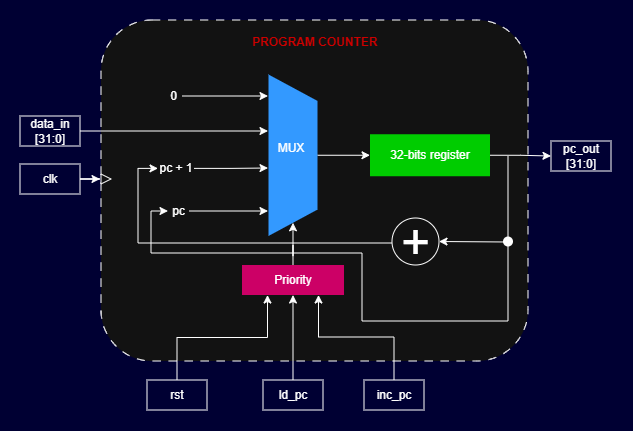
\includegraphics[width=0.8\textwidth]{PC.png} % Thay tên file sơ đồ khối PC vào đây
 \caption{Sơ đồ khối bộ đếm chương trình (PC) 32-bit}
 \label{fig:pc_32bit}
\end{figure}

\textbf{Nguyên lý hoạt động:}
Khối PC hoạt động đồng bộ theo xung lên của clk và output được chọn bởi một MUX đi kèm với một mạch ưu tiên logic. 
Khối sẽ thay đổi trạng thái dựa trên các tín hiệu điều khiển với mức độ ưu tiên từ cao xuống thấp như sau:

\begin{itemize}
 \item \textbf{Reset ($rst$):}Khi được kích hoạt, bộ đếm ngay lập tức bị xóa về giá trị 0 ($PC = 0$), đưa chương trình về trạng thái khởi tạo.
 \item \textbf{Nạp địa chỉ mới ($ld\_pc$):} Được sử dụng khi thực thi lệnh rẽ nhánh (như lệnh JMP). 
 PC sẽ nạp trực tiếp một địa chỉ 32-bit từ đầu vào ($PC = data\_in$).
 \item \textbf{Tăng bộ đếm ($inc\_pc$):} Ở trạng thái bình thường, bộ đếm sử dụng bộ cộng (Adder) 
 để tự động tăng giá trị hiện tại lên 1 đơn vị ($PC = PC + 1$), giúp CPU trỏ tới lệnh tiếp theo.
 \item \textbf{Giữ nguyên trạng thái:} Nếu không có tín hiệu nào trong ba tín hiệu trên được kích hoạt, PC sẽ duy trì giá trị địa chỉ hiện tại.
\end{itemize}